%%%%%%%%%%%%%%%%%%%
%% KAPITEL Intro %%
%%%%%%%%%%%%%%%%%%%
%% JONAS         %%
%%%%%%%%%%%%%%%%%%%
\section{Einführung}

\gls{sap} \gls{byd} ist die \gls{erp} \gls{ondemand} Cloudlösung für \gls{sme} (\ref{sec:byd}).

Für Installation, Wartung und Aktualisierung der Lösung sorgt das integrierte Betriebsmodell. Alle Betriebskosten, die durch ein Vor-Ort System entstehen sind also im Preis einbegriffen. Damit kann sich der Kunde vollständig auf sein Kerngeschäft konzentrieren.

\gls{sap} \gls{byd} wird über eine sichere Internetverbindung und einen Webbrowser als dynamische Website aufgerufen. Somit können User von überall auf ihren Arbeitsplatz zugreifen und müssen weder vor Ort im Büro sein noch sich anderweitig ins Firmennetz einwählen.

\subsubsection{Vorteile von \gls{byd}}

\begin{itemize}
\item \gls{byd} vereinigt alle Vorteile einer modernen Unternehmensanwendung bei minimalen Anforderungen an die IT
\item \gls{byd} greift auf bewährte Geschäftsvorfälle zu, die umgehend einsatzbereit sind
\item Der Kunde hat automatisch Zugriff auf die aktuellste Softwareversion des Produkts
\item \gls{byd} schont die Investition für eine eigene IT-Infrastruktur durch ein skalierbares Mietmodell
\item Die Lösung kann leicht an wechselnde Geschäftsanforderungen angepasst werden.
\end{itemize}
\cite{itelligence}

%%%%%%%%%%%%%%%%%%%%%%%%%%%%%%%%
%% KAPITEL Benutzeroberfläche %%
%%%%%%%%%%%%%%%%%%%%%%%%%%%%%%%%
%% JONAS                      %%
%%%%%%%%%%%%%%%%%%%%%%%%%%%%%%%%
\section{Benutzeroberfläche}

\begin{figure}[H]
	\begin{center}
	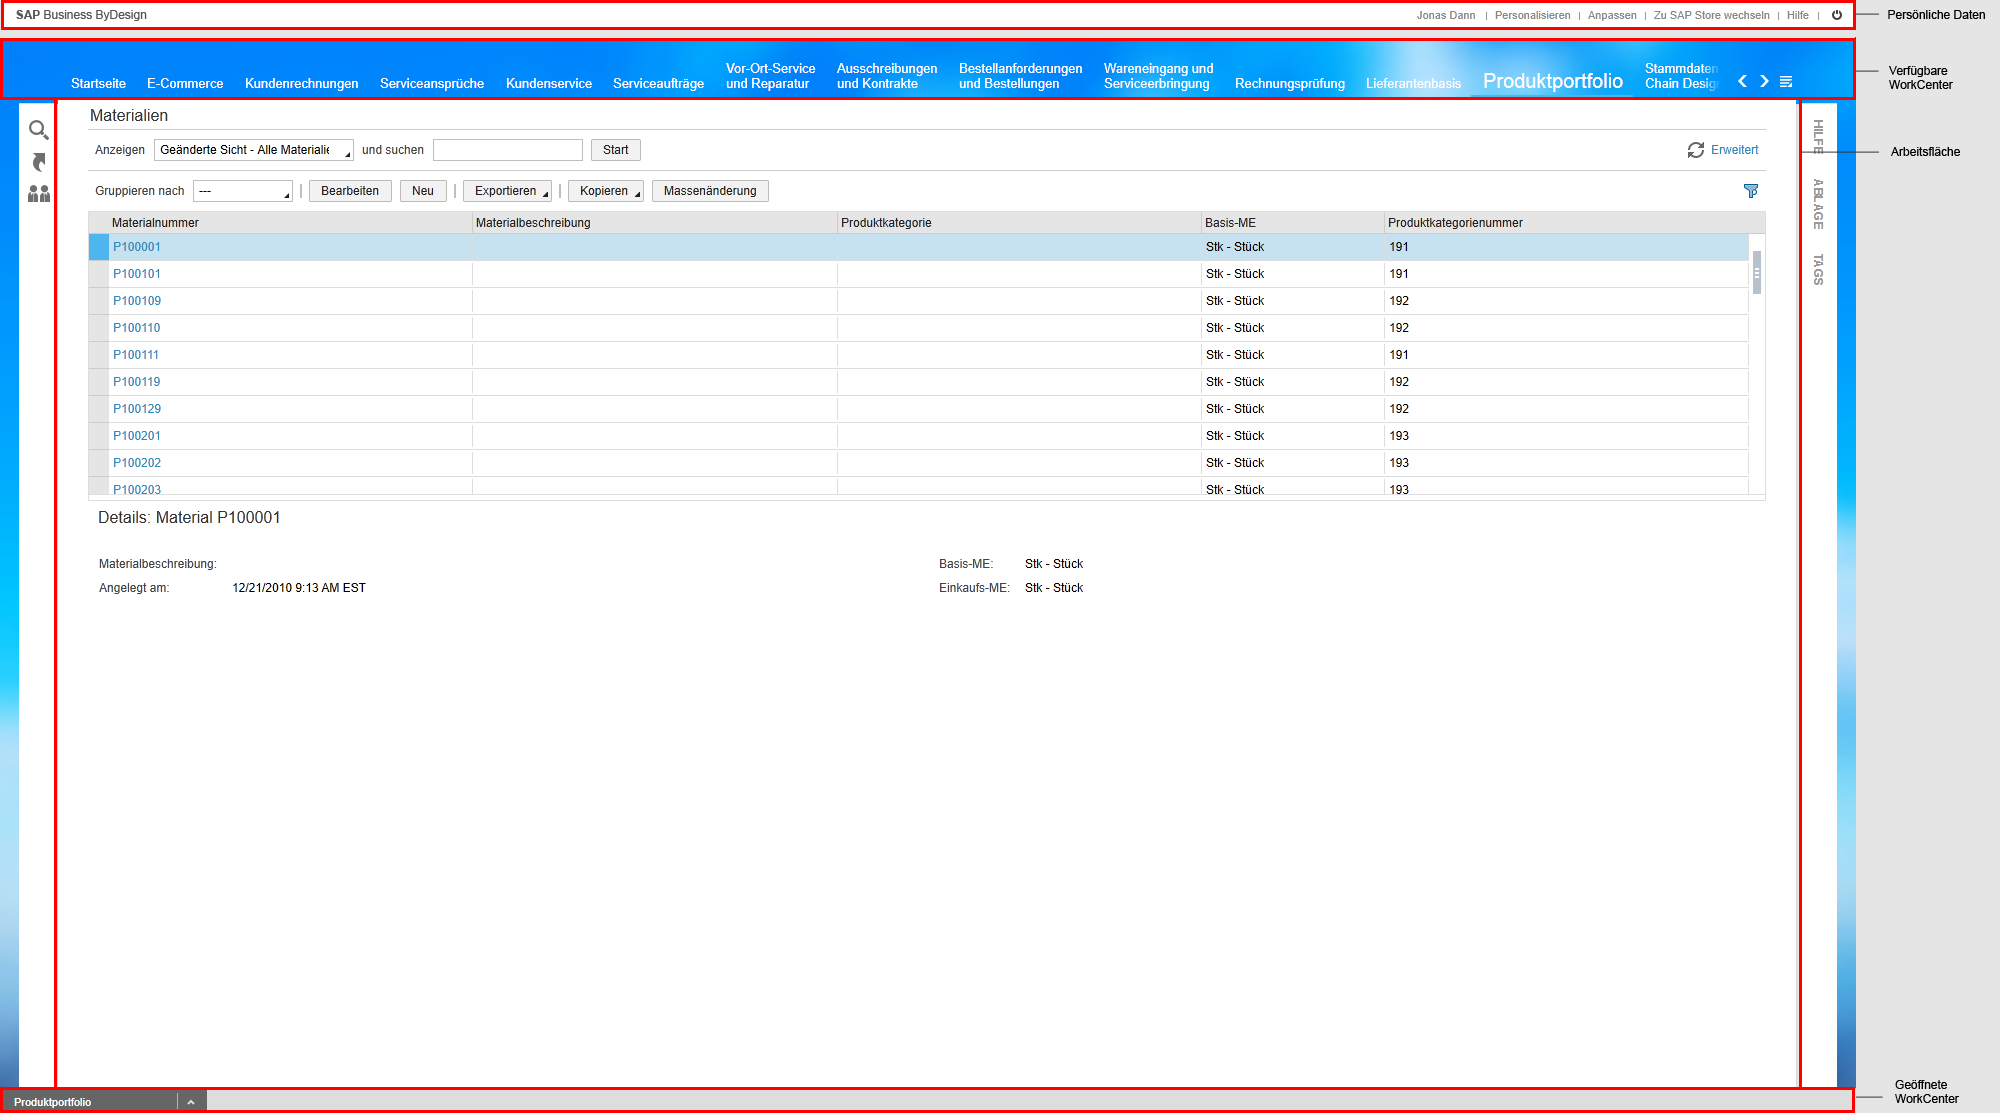
\includegraphics[width=1.0\textwidth]{grafiken/ByDesign-Ubersicht.png}
	\caption{ByDesign Übersicht}
	\vspace{-10pt}
	\label{abb:byd-overview}
	\end{center}
\end{figure}

\subsubsection{Persönliche Daten}

Hier kann der User seine Daten, wie \gls{zb} Telefonnummer oder E-Mail, einstellen. Außerdem kann er seine Benutzeroberfläche in \gls{byd} personalisieren. Weiterhin besteht die Möglichkeit in den \gls{sap}-Store zu wechseln und eine Hilfsseite aufzurufen.

\subsubsection{Verfügbare WorkCenter}

\gls{byd} ist in verschiedene WorkCenter unterteilt, die jeweils einen Teilgeschäftsprozess abbilden. So kann man \gls{zb} seine Mitarbeiter oder Waren verwalten.

In dieser Sektion der Anzeige kann der User die verschiedenen für ihn verfügbaren WorkCenter auswählen. Diese werden dann unten im "`Geöffnete WorkCenter"' Bereich angezeigt und in der Arbeitsfläche geöffnet.

\subsubsection{Arbeitsfläche}

Hier werden die eigentlichen Inhalte des Webinterfaces angezeigt. Wenn der Beispielworkflow durchgespielt wird, werden auch nur noch diese Ausschnitte des Bildschirms gezeigt.

\subsubsection{Geöffnete WorkCenter}

Im Bereich "`Geöffnete WorkCenter"' sieht der User alle WorkCenter, die er im Moment geöffnet hat. Die Anzeige funktioniert wie Tabs in einem Webbrowser und der Nutzer kann damit zwischen verschiedenen Ansichten und Aufgaben wechseln.

%%%%%%%%%%%%%%%%%%%%%%%%%%%%%%
%% KAPITEL Beispielworkflow %%
%%%%%%%%%%%%%%%%%%%%%%%%%%%%%%
%% JONAS                    %%
%%%%%%%%%%%%%%%%%%%%%%%%%%%%%%
\section{Beispielworkflow}

\subsection{Vorstellung des Workflows}
\label{sec:byd-bsp-vorstellung}
% Schulungsworkflow beschreiben (anwendersicht)

\subsubsection{Szenario}

Der Verkaufsbereichsleiter einer Firma hat auf einer Technologiemesse ein innovatives Produkt entdeckt. Er würde gerne einen neuartigen Solarboiler in das Produktportfolio der Firma aufnehmen. Die Nachfrage nach Innovation und neuen Produkten ist sehr groß.

\subsubsection{Aufgaben des Mitarbeiters}

\begin{enumerate}
 \item Er sucht einen Anbieter für das gewünschte Produkt.
 \item Danach ermittelt er über Preisvergleiche die günstigsten Anbieter, die gleichzeitig auch eine hohe Verfügbarkeit gewährleisten sollen.
 \item Er fügt das Produkt in \gls{byd} ein und ordnet ihm eine Produktkategorie zu.
 \item Nach der Zuordnung müssen alle wichtigen Daten in das System eingepflegt werden.
 \item Nun fügt er die erforderlichen Angaben über jeden Anbieter in \gls{byd} ein.
 \item Nachdem er die Anbieter angelegt hat, fordert er Angebote an.
 \item Nach Erhalt werden diese in \gls{byd} eingepflegt.
 \item Es können dann die Angebote verglichen werden und gegebenenfalls wird der Zuschlag erteilt und ein Vertrag geschlossen.
 \end{enumerate}

\subsection{Umsetzung des Workflows}
\label{sec:byd-bsp-umsetzung}
% technische sicht, "`klickbares"' howto

\subsubsection{Anbietersuche}

Im ersten Schritt werden Anbieter des gewünschten Produktes \gls{zb} auf der Website Alibaba\footnote{\url{alibaba.com}} gesucht. Auf dieser Website können kleine Unternehmer ihre Produkte zum Verkauf anbieten. Im Moment sind über 2 Millionen Anbieter registriert.

Für dieses Beispiel wird der SunSurf SC-IP01\footnote{\url{http://www.alibaba.com/product-detail/SunSurf-SC-IP01-solar-boiler-system_627442099.html?s=p}} Solar Boiler verwendet. Dieser kostet zwischen 400 und 500 USD(\$) und muss mindestens zu 15 Stück bestellt werden. Der Anbieter kann maximal 5000 Stück im Monat liefern.

\subsubsection{Produkt im System anlegen}

Im WorkCenter "`Produktportfolio"' können nun die Daten des SunSurf SC-IP01 unter einem neuen Material abgespeichert werden. Dazu klickt der User auf "`Produkte nach Materialien"' und dann auf "`Neu"'. In dem folgenden Formular werden dann die Daten des Solar Boilers angegeben (Abbildung \ref{abb:byd-newmaterial}).

Nachdem auf "`Sichern und schließen"' geklickt wurde, wurde das Produkt erfolgreich angelegt.

\subsubsection{Anbieter anlegen}

Im WorkCenter "`Lieferantenbasis"' unter "`Lieferanten"' legt der User einen neuen Anbieter an. Dazu klicken er wieder auf "`Neu"' und gibt dann im Formular die Daten des Anbieters ein (Abbildung \ref{abb:byd-newsupplier}).

Nachdem er auf "`Sichern und schließen"' geklickt hat wurden die Eingaben erfolgreich angelegt.

\subsubsection{Angebotsanforderung versenden}

Es ist alles vorbereitet um eine Ausschreibung zu erstellen. Dies geschieht im WorkCenter "`Ausschreibungen und Kontrakte"'. Dort wählt der User "`Ausschreibungen und Angebote"' aus. Er klickt auf "`Neu"' und füllen die allgemeinen Daten der Ausschreibung (Abbildung \ref{abb:byd-rfq-1}). 

Danach können die Produkte hinzugefügt werden, die mit der Ausschreibung behandelt werden sollen (Abbildung \ref{abb:byd-rfq-2}).

Als letztes fügt der Nutzer die Bieter ein, die automatisch über ihre Teilnahme an der Ausschreibung benachrichtigt werden (Abbildung \ref{abb:byd-rfq-3}).

\subsubsection{Angebot entgegennehmen}

Wenn die Bieter Angebote vorlegen, können diese über eine Eingabemaske in \gls{byd} eingegeben werden (Abbildung \ref{abb:byd-rfq-4}). Dabei werden allgemeine Daten und Preise des Bieters eingepflegt werden (Abbildung \ref{abb:byd-rfq-5}).

\subsubsection{Vertrag/Kontrakt schließen}

Sämtliche Angebote können in einer Gesamtansicht angezeigt und verglichen werden (Abbildung \ref{abb:byd-rfq-6}). Dem besten Angebot wird der Zuschlag erteilt. 
Die Entscheidung erscheint auf dem Arbeitsplatz des Vorgesetzten als offene Aufgabe. Dieser kann den Kontrakt dann schließen oder ablehnen (Abbildung \ref{abb:byd-contract}).

%%%%%%%%%%%%%%%%%%%%%
%% KAPITEL Grenzen %%
%%%%%%%%%%%%%%%%%%%%%
%% JONAS           %%
%%%%%%%%%%%%%%%%%%%%%
\section{Grenzen von ByD}

\subsubsection{Vordefinierte Geschäftsprozesse}

Die Idee eine vorkonfigurierte On-Demand Unternehmensmanagement Applikation weist Nachteile gegenüber den anderen \gls{sme}-Lösungen im Bereich Customizing auf. So kann \gls{byd} nicht beliebig granular konfiguriert werden, da die Geschäftsabläufe von \gls{sap} standardisiert vorgegeben werden.

\subsubsection{Module}

Da \gls{byd} in Form von Modulen zusammengestellt ist, erhält der Kunde unausweichlich auch Funktionalität, die er nicht nutzt und bezahlt damit für unnötige Anwendungsbestandteile. In diesem Aspekt sind Business One \ref{sec:business-one} oder \gls{sap} All-in-One \ref{sec:allinone} die bessere Wahl.

\subsubsection{Erweiterbarkeit}

Im Gegensatz zu den beiden anderen \gls{sme}-Systemen kann \gls{byd} nicht beliebig erweitert werden. So können nicht einfach spezifische Prozesse neu entwickelt und in das vorhandene System eingebunden werden, da \gls{byd} keine Möglichkeit bietet eigene Workflows anzulegen und auch \gls{sap} keine weit über die Standardsoftware hinausgehenden Add-Ons anbietet.

